\documentclass[12pt]{article}

% Importando Config
\usepackage[spanish]{babel}
\usepackage{apacite}

\addto\captionsspanish{%
  \renewcommand{\tablename}{Tabla}
}

\usepackage[table,xcdraw]{xcolor}

\usepackage[T1]{fontenc}
% \usepackage{uarial}
% \renewcommand{\familydefault}{\sfdefault}

\usepackage{etoolbox}
\patchcmd{\thebibliography}{\section*{\refname}}{}{}{}


\usepackage{url}
\def\UrlBreaks{\do\/\do-}

\usepackage{adjustbox}
\usepackage{graphicx}
\usepackage{tabularx}
\usepackage{svg}
\usepackage{float}
\restylefloat{table}

\usepackage{enumitem}

\usepackage{multicol}

\parskip=12pt 
\parindent=0pt

\usepackage{ragged2e}
\tolerance=1
\emergencystretch=\maxdimen
\hyphenpenalty=10000
\hbadness=10000
\raggedright

\usepackage{textcase}
\usepackage{tocloft}
\makeatletter
\patchcmd{\l@section}{#1}{\MakeTextUppercase{#1}}{}{}
\patchcmd{\l@subsection}{#1}{\MakeTextUppercase{#1}}{}{}
\patchcmd{\l@subsubsection}{#1}{\MakeTextUppercase{#1}}{}{}
\makeatother

\usepackage{titlesec}
\titleformat{\section}{\raggedright\normalfont\normalsize\bfseries\uppercase}{\thesection}{1em}{}
\titleformat{\subsection}{\raggedright\normalfont\normalsize\bfseries\uppercase}{\thesubsection}{1em}{}
\titleformat{\subsubsection}{\raggedright\normalfont\normalsize\bfseries\uppercase}{\thesubsubsection}{1em}{}

\usepackage{geometry}
\geometry {
    letterpaper,
    left = 1in,
    right = 1in,
    bottom = 1in,
    top = 1in
}

% Line break
\newcommand{\skipline}{\par\null\par}

\usepackage{subfig}

\newcommand*{\Universidad}[1]{\def\Uni{#1}}
\newcommand*{\Facultad}[1]{\def\Fac{#1}}
\newcommand*{\Escuela}[1]{\def\Esc{#1}}

\usepackage{datetime}
\newdateformat{daymonthyear}{\THEDAY \ de \monthname[\THEMONTH] de \THEYEAR}
\newcommand*{\CiudadFecha}{Bucaramanga, \daymonthyear\today }

\newcommand*{\Titulo}[1]{\def\Tit{#1}}
\newcommand*{\Modalidad}[1]{\def\Mod{#1}}
\newcommand*{\Autor}[2]{\def\Nam{#1}\def\Cod{#2}}
\newcommand*{\Director}[3][]{\def\TDir{#1}\def\Dir{#2}\def\EDir{#3}}
\newcommand*{\CoDirector}[3][]{\def\TCDir{#1}\def\CDir{#2}\def\ECDir{#3}}
\newcommand*{\EntidadInt}[1]{\def\EntI{#1}}

\newcommand*{\captionsource}[2]{%
  \caption[{#1}]{%
    #1%
    \\\hspace{\linewidth}%
    \textbf{Source:} #2%
  }%
}

\titlespacing\section{0pt}{12pt plus 4pt minus 2pt}{0pt plus 2pt minus 2pt}
\titlespacing\subsection{0pt}{12pt plus 4pt minus 2pt}{0pt plus 2pt minus 2pt}
\titlespacing\subsubsection{0pt}{12pt plus 4pt minus 2pt}{0pt plus 2pt minus 2pt}


\bibliographystyle{apacite}

% Definiendo constantes
\Universidad{Universidad Industrial de Santander}
\Facultad{Facultad De Ingenierías Fisicomecánicas}
\Escuela{Escuela De Ingeniería De Sistemas E Informática}
\Titulo{Mecanismos de adaptación autonómica de arquitectura software para la plataforma Smart Campus UIS}
\Modalidad{Trabajo de investigación}
\Autor{Daniel David Delgado Cervantes}{2182066}
\Director[PhD.]{Gabriel Rodrigo Pedraza Ferreira}{Escuela De Ingeniería De Sistemas e Informática}
\CoDirector[MSc.]{Henry Andrés Jiménez Herrera}{Escuela De Ingeniería De Sistemas e Informática} 
\EntidadInt{Universidad Industrial de Santander}

% En el caso de no tener codirector, quitar la linea `\textbf{CODIRECTOR: } \TCDir\ \CDir, \ECDir` de 'Sections/title.tex'

\begin{document}

    % maketitle page
    % --------------------------------------------------------------------------------------------------------- %
%                                               Section: Title                                              %
% --------------------------------------------------------------------------------------------------------- %

\renewcommand{\contentsname}{\hfill\bfseries\normalsize \MakeUppercase{Tabla de Contenido}\hfill}
\renewcommand{\cftaftertoctitle}{\hfill}

\begin{titlepage}
        
    \begin{center}

        \textbf{\MakeUppercase{\Uni}} \\
        \textbf{\MakeUppercase{\Fac}} \\
        \textbf{\MakeUppercase{\Esc}}
        
        \skipline
        
        \textbf{PLAN DE TRABAJO DE GRADO}
        
        \skipline
        \skipline
        
    \end{center}
    
    
    \textbf{FECHA DE PRESENTACIÓN: } \CiudadFecha

    \textbf{TÍTULO: } \Tit
    
    \textbf{MODALIDAD: } \Mod

    \textbf{AUTOR: } \Nam, \Cod

    \textbf{DIRECTOR: } \TDir\ \Dir, \EDir
    
    \textbf{CODIRECTOR: } \TCDir\ \CDir, \ECDir

    \textbf{ENTIDAD INTERESADA: } \EntI 
    
\end{titlepage}

\tableofcontents

\pagebreak
\begin{center}
    \MakeUppercase{\textbf{ \Tit}}
\end{center}
    
    \section{Introducción}

    % 1. Origen de la computación autonómica (Citation needed for industry tendencies)

    La computación autonómica, concebida inicialmente por IBM en el año 2001, se refiere al uso de sistemas auto-gestionados con la capacidad de operar y adaptarse sin la intervención de un ser humano. En este sentido, este acercamiento tiene como objetivo la creación de sistemas computacionales capaces de reconfigurarse en respuesta a cambios en las condiciones del entorno al igual que los objetivos del negocio \cite{horn_2001}.

    % Esta autonomía es adquirida con el uso de ciclos de control, en el caso de la computación autonómica, de los ciclos más populares es el ciclo MAPE-K \cite{Arcaini_2015}. Estos le dan la capacidad al sistema de monitorear tanto su estado actual como el entorno en el que este se encuentra, analizar la información recolectada para luego planear y ejecutar los cambios requeridos sobre el sistema \cite{RutanenKalle2018McoO}.
    
    En la última década, el interés de la computación autonómica ha ido en 2 direcciones. Aunque la investigación y la cantidad de artículos ha ido bajando (Ver figura \ref{fig:scopus}), es posible ver el cómo las patentes se han ido manteniendo relativamente estables (Ver figura \ref{fig:lens}). Aunque esto puede representar un interés más hacia el desarrollo de productos derivados de los estudios de la computación autonómica, sugiere que aún existe un atractivo dentro de la investigación en pro del desarrollo de productos. 

    \begin{figure}[h]
        \centering
        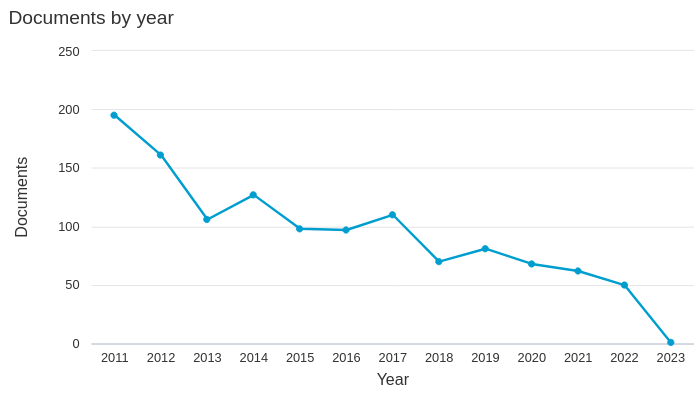
\includegraphics[scale=0.5]{Images/Scopus.png}
        \caption{Documentos publicados sobre computación autonómica desde 2011 hasta 2023} \cite{scopus} 
        \label{fig:scopus}
    \end{figure}

    \begin{figure}[h]
        \centering
        \includesvg[inkscapelatex=false, scale=0.5]{Images/lens.svg}
        \caption{Patentes sobre computación autonómica desde 2011 hasta 2023} \cite{lens} 
        \label{fig:lens}
    \end{figure}

    % 2. Relación y utilidad para las otras ramas de la computación (¿Qué ramas?, ¿Por qué les es útil?)

    Una de las áreas que pueden verse especialmente beneficiadas de la computación autonómica es la del internet de las cosas (IoT). Esto se debe a tanto la gran cantidad de dispositivos a manejar al igual que la complejidad que es darles un mantenimiento debido a la distribución geográfica de estos \cite{Tahir_2019}. 
    
    Esto puede verse el Smart Campus UIS, una plataforma IoT de la Universidad Industrial de Santander, que permite usar dispositivos con el fin de monitorear y recolectar de información en tiempo real con el objetivo de apoyar la toma de decisiones, mejora de servicios, entre otros \cite{henry_2020}.

    Ahora, esta plataforma ha tenido esfuerzos en el desarrollo de características propias de un sistema autonómico. Uno de estos ha sido la integración de mecanismos para la auto-descripción de la estructura de los sistemas IoT conectados a la plataforma al igual la capacidad de adaptar la arquitectura \cite{henry_2020}. %!!! Arreglar esto, no tengo la referencia correcta porque eso es de la tesis de maestría de Henry !!!%
    
    % 4. Presentar el objetivo final del proyecto (¿Qué se espera obtener?)

    Partiendo de lo anterior, y con la intención de dar continuidad con los esfuerzos de desarrollo realizados en la plataforma Smart Campus UIS, se plantea como caso de estudio iterar sobre la implementación de mecanismos de adaptación realizada, mejorando la manera en la que estos puedan alterar el estado de la plataforma a partir de un objetivo establecido.  

    % 5. Presentar de manera general la metodología a seguir

    \section{Planteamiento Y Justificación Del Problema}
    
    % La complejidad de los sistemas software ha ido en aumento \cite[pp.~4-5]{horn_2001}. A medida que se hace la transición a arquitecturas orientadas a microservicios \cite{forrester_research_2019}; la computación distribuida es más común gracias a las soluciones \textit{cloud} \cite{the_cloud_in_2021} y la computación embebida se hace más presente en la industria y el día a día \cite{deichmann_2022}; la administración y gestión de estos requiere de una mayor cantidad de recursos en términos técnicos y humanos con el fin de mantenerlos en los estados más óptimos respecto a los requerimientos del negocio. La búsqueda de reducir o abstraer la complejidad de la gerencia de estos sistemas se ha convertido en una necesidad \cite{lalanda_diaconescu_mccann_2014}.
    
    % Una de las posibles soluciones se encuentra en la computación autonómica. Desde este enfoque, se tiene como objetivo sistemas con la capacidad de auto-gestión, es decir, sistemas con la capacidad de manejarse a ellos mismos dependiendo de las necesidades y las metas establecidas por los administradores del sistema \cite{evaluation_2004}. 

    El crecimiento de las capacidades de los sistemas de software en términos de la escala, tienen como consecuencia el aumento en la complejidad, heterogeneidad e incertidumbre \cite{emerging_2005}. El manejo de una gran cantidad de estos componentes es un reto en términos de recursos técnicos y humanos \cite[pp.~4-5]{horn_2001}. 
    
    Una de las posibles maneras de dar solución a esta problemática, en cuanto al manejo de sistemas, está en el área de la computación autonómica. Este acercamiento basado en conceptos biológicos busca solventar los problemas de complejidad, heterogeneidad e incertidumbre \cite{emerging_2005} a partir de la abstracción de las metas de los administradores y delegación del manejo del sistema a sí mismo \cite{lalanda_diaconescu_mccann_2014}.
    
    La propuesta de IBM, responsables de los primeros acercamientos a la computación autonómica, es especialmente interesante en los casos de las arquitecturas de software orientadas a microservicios, uno de los patrones de diseño más usados \cite{forrester_research_2019}; al igual los sistemas embebidos se hacen más presentes en la industria \cite{deichmann_2022}; los cuales afrontan una gran cantidad de incertidumbre. 
    
    Considerando lo anterior, una de las aplicaciones de los sistemas está en la IoT y los Smart Campus, una variación de las Smart Cities en las cuales se busca la recolección de información y monitoreo en tiempo real con el fin de apoyar la toma de decisiones, mejora de servicios, entre otros \cite{MinAllah2020}. Es en este tipo de aplicaciones, debido incertidumbre generada por la cantidad de componentes distribuidos en puntos geográficamente apartados, que la computación autonómica se presenta un gran potencial. 

    Dentro del marco del presente proyecto, se tiene Smart Campus UIS, una plataforma de IoT de la Universidad Industrial de Santander, en la cual se han realizado implementaciones parciales de una arquitectura autonómica con capacidad de auto-describirse al igual que un avance a la auto-sanación \cite{henry_2020}, características principales de un sistema autonómico \cite{horn_2001}. 
    
    Dicho esto, y con la intención de dar continuidad con los esfuerzos de desarrollo realizados en la plataforma, se plantea como caso de estudio la implementación de mecanismos de adaptación con los cuales se pueda alterar el estado de la plataforma a partir de un objetivo establecido.  


    \section{Objetivos}
    \subsection{Objetivo General}
    \begin{itemize}

        \item Implementar un conjunto de mecanismos autonómicos para permitir la adaptación de la Arquitectura Software IoT respecto a un modelo objetivo en la plataforma Smart Campus UIS

    \end{itemize}

    \subsection{Objetivos Específicos}

    \begin{itemize}
        \item Proponer una notación (lenguaje) para describir una arquitectura objetivo de un sistema software IoT.
        \item Diseñar un mecanismo para determinar las diferencias existentes entre una arquitectura actual en ejecución y una arquitectura objetivo especificada.
        \item Diseñar un conjunto de mecanismos de adaptación que permitan disminuir las diferencias entre la arquitectura actual y la arquitectura objetivo.
        \item Evaluar la implementación realizada a partir de un conjunto de pruebas con el fin de establecer la efectividad de los mecanismos usados.

    \end{itemize}


    \section{Marco De Referencia}

    Como base para el desarrollo del proyecto es necesario establecer los fundamentos para la selección de los mecanismos de adaptación, por lo cual es indispensable conocer los principios de la computación autonómica, las aplicaciones de la misma en la industria y las partes requeridas para la integración, las cuales se describen a continuación.

    \subsection{Computación Autonómica}
    
    % Definir qué es la computación autonómica y qué es lo que propone

    El concepto de computación autonómica, definido inicialmente por IBM \citeyear{horn_2001}, se refiere a un conjunto de características que presenta un sistema computacional el cual le permite actuar de manera autónoma, o auto-gobernarse, con el fin de alcanzar algún objetivo establecido por los administradores del sistema \cite{lalanda_diaconescu_mccann_2014}.


    Los 8 elementos clave, definidos por IBM, que deberían presentar este tipo de sistemas son:
    % \begin{multicols}{2}
    \begin{enumerate}
        \item Auto-conocimiento: habilidad de conocer su estado actual, las interacciones del sistema.
        \item Auto-configuración: capacidad de reconfigurarse frente a los constantes cambios en el entorno.
        \item Auto-optimización: búsqueda constante de optimizar el funcionamiento de sí mismo.
        \item Auto-sanación: aptitud de restaurar el sistema en el caso de que se presenten fallas.
        \item Auto-protección: facultad de protegerse a sí mismo de ataques externos.
        \item Auto-conciencia: posibilidad de conocer el ambiente en el que el sistema se encuentra.
        \item Heterogeneidad: capacidad de interactuar con otros sistemas de manera cooperativa.
        \item Abstracción: ocultar la complejidad a los administradores del sistema con objetivos de alto nivel de abstracción.
    \end{enumerate}
    % \end{multicols}

    En el caso de que un sistema tenga una implementación parcial de estas características, este podría considerarse autonómico. En este sentido debería tener la capacidad de lidiar con los problemas como la complejidad, heterogeneidad e incertidumbre \cite{emerging_2005} al igual que reducir la cantidad de recursos tanto técnicos como humanos requeridos para mantener los sistemas en funcionamiento.
    
    \subsubsection*{MAPE-K}

    % Explicar como funciona el modelo de management y los pasos que se aplican dentro de lo que se tiene
    % Más que todo es desarrollar que es el ciclo MAPE-K

    IBM, en cuanto a la implementación de las características, propone una modelo de ciclo auto-adaptativo, denominado MAPE-K \cite{Krikava2013}. Este acercamiento, compuesto de cinco fases, es uno de ciclos de control más usado en implementaciones de sistemas auto-adaptativos y computación autonómica \cite{Arcaini_2015}. En la figura \ref{fig:mapek}, se presentan las fases que \textit{manejador} debe desarrollar para así administrar cada uno de los elementos del sistema computacional basado en una base de conocimiento común \cite{alessandra_2010}. 

    \begin{figure}[H]
        \centering
        \includesvg[inkscapelatex=false]{Images/Mape-k.svg}
        \caption{El ciclo auto-adaptativo MAPE-K.} \cite{alessandra_2010}
        \label{fig:mapek}
    \end{figure}

    Cada una de estas fases son:

    \begin{itemize}
        \item Monitorear (M): Esta fase se compone de la recolección, filtración y reportar la información adquirida sobre el estado del elemento a manejar.
        \item Analizar (A): La fase de análisis se encarga del interpretar el entorno en el cual se encuentra, el predecir posibles situaciones comunes y diagnosticar el estado del sistema.
        \item Planear (P): Durante la planificación se determina las acciones a tomar con el fin de llegar a un objetivo establecido a partir de una serie de reglas o estrategias.
        \item Ejecutar (E): Finalmente, se ejecuta lo planeado usando los mecanismos disponibles para el manejo del sistema. 
    \end{itemize}

    Es de resaltar que este modelo, aunque útil para el desarrollo de este tipo de sistemas, es bastante general en cuanto a la estructura y no usan modelos de diseño establecidos \cite{Ouareth_2018}. 

    \subsubsection*{Mecanismos de Descripción}

    % Esta parte está más que todo para introducir el concepto de la base de conocimiento de la aplicación.
    % Es decir, está orientado a dar como un ejemplo de esa base de conocimiento que tiene el "manejador" sobre la 
    % plataforma

    La fase de monitoreo dentro del ciclo MAPE-K es vital para el funcionamiento del manejador autonómico pues es a partir de la información que se construirá la base de conocimiento requerida por las demás partes del ciclo. Parte de esta, está compuesta por el \textit{estado del sistema} el cual incluye la descripción del sistema en un momento dado \cite{Weiss_2011}.

    Existen varias maneras de realizar implementaciones de mecanismos de auto-descripción y la utilidad de cada uno de estos varía dependiendo en el tipo de sistema de software que se esté usando. Para el marco del proyecto, nos interesan aquellos que estén orientados a los sistemas embebidos e  IoT, algunos de estos son:
    
    \begin{itemize}
        \item \textbf{JSON Messaging}: Iancu y Gatea \citeyear{Iancu_2022} plantean un protocolo que emplea mensajería entre \textit{gateways} con el fin de recibir información sobre estas. En términos simples, estas funcionan como un \textit{ping} hacia el nodo que luego retorna sus datos, al igual que los dispositivos conectados a ella, al encargado de recolectar toda esta información con el fin de construir una descripción del sistema.-
        
        \item \textbf{IoT Service Description Model}: O IoT-LMsDM, es un servicio de descripción desarrollado por Zhen y Aiello \citeyear{Wang_2021} el cual está orientado al contexto, servicios e interfaz de un sistema IoT. De este se espera poder contar no solo con descripciones del estado del sistema en términos del ambiente, pero la funcionalidad (es decir, los \textit{endpoints} a usar) al igual que las estructuras de datos que estos consumen.
        
        \item Henry!!!
    \end{itemize}

    De esto podemos ver no solo las diferentes maneras en las que las implementaciones realizan las descripciones de los sistemas asociados, sino que también el alcance de estos en cuanto a lo que pueden describir.
    
    \subsubsection*{Mecanismos de Adaptación}
    
    % Ya aquí es como definir de manera general qué es eso de los mecanismos de adaptación, qué hacen y qué características
    % tienen. 
    % No sé si meter ejemplos, creo que eso sería más para un estado del arte en este caso.

    La adaptación, en el contexto de la computación autonómica, es la parte más importante en cuanto a la auto-gestión de un sistema de software se refiere. Así mismo, presenta el mayor reto debido a la necesidad de modificar código de bajo nivel, tener que afrontarse a incertidumbre de los efectos que pueden tener dichas alteraciones al sistema al igual que lidiar con esto en \textit{runtime} debido a los problemas que el \textit{downtime} tendría en los negocios \cite{lalanda_diaconescu_mccann_2014}. 
    
    Esta adaptabilidad puede exponerse en múltiples puntos dentro de un sistema de software. Pueden realizarse adaptaciones en sistema operativo, lenguaje de programación, arquitectura e incluso datos \cite{lalanda_diaconescu_mccann_2014}. 

    Manteniéndose en el marco del proyecto, son las implementaciones relacionadas con la modificación de la arquitectura los cuales nos interesan. Siendo así, nos centraremos en los mecanismos de adaptación de componentes, o de reconfiguración:

    \begin{itemize}
        \item \textbf{Binding Modification}: Este mecanismo hace referencia a la alteración de los vínculos entre los diferentes componentes de la arquitectura. Estos tienen el objetivo de modificar la interacción entre componentes, lo que es especialmente común en implementaciones con \textit{proxies}. Este tipo de mecanismo de adaptación fue usado por Kabashkin \citeyear{Kabashkin_2017} para añadir fiabilidad a la red de comunicación aérea.

        \item \textbf{Interface Modification}: Las interfases funcionan como los puntos de comunicación entre los diferentes componentes de la arquitectura. Siendo así, es posible que la modificación de estos sea de interés con el fin de alterar el comportamiento de un sistema al igual que soportar la heterogeneidad del sistema. Esto puede verse en el trabajo desarrollado por Liu, Parashar y Hariri \citeyear{Liu_2004} en donde definen la utilidad de dichas adaptaciones al igual que la implementación de las mismas.

        \item \textbf{Component Replacement, Addition and Subtraction}: En términos simples, este mecanismo se encarga de alterar los componentes que componen la arquitectura; de esta manera, modificando su comportamiento. Ejemplos de esto puede verse en el trabajo de Huynh \citeyear{Huynh_2019} en el cual se evalúan varios acercamientos a la reconfiguración de arquitecturas a partir del remplazo de componentes a nivel individual al igual que grupal. 
        
        Este acercamiento a la mutación de la arquitectura también puede verse en el despliegue de componentes como respuesta a cambios en los objetivos de negocio de las aplicaciones al igual que como respuesta a cambios inesperados dentro de la aplicación. Esto puede verse en trabajos como el de Patouni \citeyear{Patouni_2006} donde se realizan este tipo de implementaciones. %% !!! Henry puede servirme aquí por la implementación que se hizo en Smart Campus

    \end{itemize}

    \subsection{Sistemas Embebidos}
    
    % Tengo que contextualizar qué es lo que es la computación embebida y cual es el principio o justificación de este

    Los sistemas de cómputo embebidos, o simplemente sistemas embebidos, hacen referencia a un sistema compuesto de microcontroladores los cuales están orientados a llevar a cabo una función o un rango de funciones específicas \cite{heath2002embedded}. Este tipo de sistemas, debido a la posibilidad de combinar hardware y software en una manera compacta, se ha visto en multiples campos de la industria como lo son el sector automotor, de maquinaria industrial o electrónica de consumo \cite{deichmann_2022}.

    % Extender la aplicación de la computación autonómica en los sistemas embebidos.

    \subsubsection*{Internet of Things}

    % Aquí es para contextualizar una de las aplicaciones de la computación embebida más que otra cosa

    El Internet de las cosas, o IoT; es una de las sub-ramas de los sistemas embebidos. En esta, se embeben diferentes dispositivos en objetos del día a día. Esto les da la capacidad de enviar y recibir información con el fin de realizar monitoreo o facilitar el control de ciertas acciones \cite{Berte_2018}.

    Esta tecnología, debido a su flexibilidad al igual que el alcance que puede tener, presenta una gran cantidad de aplicaciones que va desde electrónica de consumo hasta la industria. Encuestas realizadas en el 2020 reportan su uso en smart homes, smart cities, transporte, agricultura, medicina, etc. \cite{Dawood_2020}. Su impacto no ha sido poco.

    % !!!

    \subsubsection*{Smart Campus}

    % Y aquí es para explicar el concepto de un smart campus. Para qué se usa y de donde surge.

    Un Smart Campus, equiparable con el concepto de Smart City, es una plataforma en la que se emplean tecnologías, sumado a una infraestructura física, con la cual se busca la recolección de información y monitoreo en tiempo real \cite{MinAllah2020}. Los datos recolectados tienen el objetivo de apoyar la toma de decisiones, mejora de servicios, entre otros \cite{Anagnostopoulos_2023}.

    Estas plataformas, debido a su escala y alcance en cuanto a la cantidad de servicios que pueden ofrecer, requieren de 
    infraestructuras tecnológicas las cuales den soporte a los objetivos del sistema. Es posible ver implementaciones orientadas a microservicios en trabajos como los de Jiménez, Cárcamo y Pedraza \citeyear{henry_2020} donde se desarrolla una plataforma de software escalable con la cual se pueda lograr interoperatividad y alta usabilidad para todos.

    % !!!

    \subsection{Notación} % Fase 2

    % En esta selección es más que todo el dar el concepto de qué es un lenguaje de notación

    % Explicar que es la notación en general, en términos lingüísticos y de ahí expandir a notación en software
    % UML y eso.

    El concepto de \textit{notación} está definido como la representación gráfica del habla \cite{crystal2011dictionary}. En el contexto de las ciencias de la computación, esta idea se ha extrapolado con el fin de representar diferentes conceptos específicos del software y algoritmia de manera visual \cite{RutanenKalle2018McoO}. Esto puede verse con la existencia de lenguajes de notación como lo es UML con el cual se realizan representaciones que van desde arquitecturas de software, estructuras de base de datos, entre otros \cite{Booch2005-xu}.
    
    \subsubsection*{Gramática}

    % Esto es más que nada para contextualizar la necesidad de una forma en la notación

    La gramática, más específicamente gramáticas libres de contexto, son un conjunto de reglas descriptivas. Este conjunto de reglas, en conjunto de una notación, cumplen la función de dictar si una frase es válida para un lenguaje dado \cite[p. 101]{Sipser2012-wl}. 

    

    \subsubsection*{Serialización de Datos}

    % qué es la serialización de datos y para que se usa en el caso de las arquitecturas.

    La serialización de datos se refiere a la traducción de una estructura de datos hacia una manera en la que pueda ser almacenada. En el contexto del proyecto, esta serialización nos permitirá describir las arquitecturas objetivo a partir de la notación y gramáticas establecidas. Así mismo, debería darnos la flexibilidad de describir cualquier tipo de meta para el sistema de software.
    

    \subsection{Algoritmia de Comparación de Grafos} % Fase 3 

    % Qué y para que se usa. Más que todo como contexto de lo que vamos a usar en la fase 3 del proyecto

    % !!!

    \pagebreak

    \section{Metodología}

    Para el desarrollo del trabajo de grado, se propone un modelo de prototipado iterativo compuesto de 5 fases (Ver fig. \ref{fig:met}). De esta manera, se avanzará a medida que se va completando la fase anterior y permitirá a futuro el poder iterar sobre lo que se ha desarrollado anteriormente.

    \begin{figure}[H]
        \centering
        \includesvg{Images/DiagramaMetodologia.svg}
        \caption{Metodología del proyecto}
        \label{fig:met}
    \end{figure}

    \subsection{Ambientación Conceptual y Tecnológica}

    La primera fase de la metodología se basa en la investigación de la literatura, al igual que de la industria, necesaria para cubrir las bases tanto conceptuales como técnicas necesarias para el desarrollo del proyecto. 

    \subsubsection*{Actividades}

    \begin{enumerate}[label=\thesubsection.\arabic*., wide, labelindent=2em, leftmargin=5em]
        \item Identificación de las características principales de un sistema auto-adaptable.
        \item Análisis de los mecanismos de adaptación de la arquitectura.
        \item Análisis los algoritmos empleados para la comparación de la comparación de las arquitecturas.
        \item Determinación de los criterios de selección para el lenguaje de notación.
        \item Evaluación de los posibles lenguajes de programación para la implementación a realizar.
        \item Imprevistos.
        \item Análisis, retroalimentación y conclusiones del desarrollo de la fase. 
    \end{enumerate} 

    \subsection{Definición de la notación de la arquitectura}
    
    La segunda fase está en la definición del cómo se realiza la declaración de la arquitectura. Partiendo de los criterios de selección establecidos en la fase 1, se espera determinar un lenguaje de notación el cual nos permita definir la arquitectura objetivo a alcanzar, al igual que la gramática correspondiente para poder realizar dicha declaración. 
    
    \subsubsection*{Actividades}

    \begin{enumerate}[label=\thesubsection.\arabic*., wide, labelindent=2em, leftmargin=5em]
        \item Selección del lenguaje de marcado a usar a partir de los criterios establecidos.
        \item Definición la gramática a usar para la definición de la arquitectura.
        \item Implementación la traducción de la notación al modelo de grafos. % (¿Esto en qué fase debería estar?)
        \item Determinación como se realizará la representación de los componentes y partes de la arquitectura.
        \item Imprevistos.
        \item Análisis, retroalimentación y conclusiones del desarrollo de la fase. 
    \end{enumerate}    

    \subsection{Mecanismos De Comparación}

    Durante la tercera fase del proyecto, se buscará poder determinar e implementar cómo se realizará la comparación entre el estado de la arquitectura obtenido durante la auto-descripción de la misma y el objetivo establecido. Así mismo, y con el fin de reportar a los administradores de los sistemas, también será necesario definir \textit{niveles} de similitud entre las 2 arquitecturas.

    \subsubsection*{Actividades}

    \begin{enumerate}[label=\thesubsection.\arabic*., wide, labelindent=2em, leftmargin=5em]
        \item Selección del mecanismo de comparación a usar para evaluación de estado de la arquitectura.
        \item Implementación del mecanismo de comparación seleccionado.
        \item Determinación de los diferentes niveles de similitud entre arquitecturas.
        \item Imprevistos.
        \item Análisis, retroalimentación y conclusiones del desarrollo de la fase. 
    \end{enumerate}    

    \subsection{Mecanismos De Adaptación}
    
    La cuarta fase del proyecto está orientada a la selección, al igual que la implementación en Smart Campus UIS, del conjunto de mecanismos de adaptación de la arquitectura. 

    \subsubsection{Actividades}

   \begin{enumerate}[label=\thesubsection.\arabic*., wide, labelindent=2em, leftmargin=5em]
        \item Definición el conjunto de mecanismos de adaptación.
        \item Implementación el conjunto de mecanismos de adaptación seleccionados.
        \item Imprevistos.
        \item Análisis, retroalimentación y conclusiones del desarrollo de la fase. 
    \end{enumerate}  
    
    \subsection{Validación De Resultados}
    
    La fase final del proyecto se encargará principalmente de la realización de pruebas de los mecanismos implementados, los resultados obtenidos al igual que la documentación de todo lo que se desarrolló durante el proyecto.
    
    \subsubsection*{Actividades}
    
   \begin{enumerate}[label=\thesubsection.\arabic*., wide, labelindent=2em, leftmargin=5em]
        \item Realización de las pruebas del funcionamiento de la implementación realizada con diversas arquitecturas objetivo.
        \item Recopilación la documentación generada durante el desarrollo de cada una de las fases del proyecto.
        \item Compilación de la documentación para generar el documento de final.
        \item Correcciones y adiciones para la presentación final del proyecto de grado.
    \end{enumerate}  

    \section{Cronograma}

    Se debe realizar un cronograma que relacione las actividades prioritarias del proyecto y el tiempo que destinará a cada una de ellas. Tenga en cuenta que el semestre tiene 16 semanas y debe desarrollar todo el trabajo de grado en este tiempo. 

    \section{Presupuesto}
    
    \begin{table}[ht]
    \small
    % \resizebox{\textwidth}{!}{%
        % \begin{tabular}{|l|c|c|c|c|}
            \begin{tabularx}{\textwidth}{|X|c|X|X|X|}
                \hline
                \multicolumn{1}{|c}{\textbf{Descripción}} & \multicolumn{1}{|c}{\textbf{Responsable}} & \multicolumn{1}{|c}{\textbf{Valor}} & \multicolumn{1}{|c}{\textbf{Cantidad}} & \multicolumn{1}{|c|}{\textbf{Precio}} \\ \hline
                DIRECTOR DE PROYECTO PhD. Gabriel Rodrigo Pedraza Ferreira & UIS & COP 305.000/Hora & \multicolumn{1}{X|}{\raggedright 4 horas mensuales por 4 meses} & COP 4'880.000 \\ \hline
        &  &  &  &  \\ \hline
        &  &  &  &  \\ \hline
        &  &  &  &  \\ \hline
        &  &  &  &  \\ \hline
        
        % \end{tabular}%
        \end{tabularx}{\parfillskip=0pt\par}
    % }
    \end{table}
    

    \pagebreak

    \section{Bibliografía}

    \begingroup
    \renewcommand{\section}[2]{}
    \renewcommand{\addcontentsline}[3]{}
    \bibliography{bibliography}
    \endgroup

\end{document} 